\chapter{Operations}
\label{chapter:operations}

{\projectname} is in regular robotic operation under the responsibility of the observatory staff. Weather permitting, {\projectname} will operate from 30 minutes before sunset to the end of morning astronomical twilight.

\section{Participants}

By “observatory staff” we refer to the telescope operators, resident astronomers, and maintenance technicians. The actually division of responsibilities will be decided by the Secretario Técnico of the observatory.

By “team members” we refer to members of the {\projectname} technical teams.

\section{Communications}

Communication between the observatory staff and the team will take place primarily through the RATIR/COATLI/DDOTI operations Skype chat.

\section{Daily Operations}

The daily operating procedure is:

\begin{enumerate}

\item At the latest one hour before sunset, the observatory staff will carry out a review of the {\projectname} installation. 

This revision has three elements. The observatory staff will:

\begin{enumerate}
\item
Check that all of the control system servers are not showing errors in the web interface (see \S\ref{figure:interface-main-page}). 
\item
Check that the webcams in the web interface are not showing an unusual situation.
\item
If necessary, carry out an on-site inspection of {\projectname}. For example, after a snowfall, it might not be obvious from the webcams whether snow remains on the roof of the enclosure.
\end{enumerate}

\textcolor{red}{MAGUI: To interact with the COATLI/OAN control system, in regular robotic operation, the observatory staff will use the web interface described in section \ref{chapter:interface}.}

If the observatory staff consider that decisions to open and close the installation can be safely taken by the control system, they will enable the supervisor by pressing the “Enable” button in the “Supervisor” section of the web interface (see \S\ref{figure:interface-main-page}).

If the observatory staff considers that decisions to open and close the installation cannot be safely taken by the control system, they should explicitly force the supervisor to maintain the telescope closed by pressing the “Close” button in the “Supervisor” section of the web interface (see \S\ref{figure:interface-main-page}).. 

The observatory staff will report the result of their inspection in the Skype chat and will indicate whether they are enabling the supervisor or forcing it to close.

\item
If the supervisor is enabled and weather conditions are benign, the control system will:
\begin{enumerate}
\item
Open partially to cool about half an hour before sunset;
\item
Open completely to observe at sunset; and
\item
Close at the end of morning astronomical twilight.
\end{enumerate}

If the supervisor is enabled and weather conditions are not benign, the control system will not open (if closed) or will close (if open).

If the supervisor is enabled and weather conditions change from not benign to benign, the control system will open partially to cool (between half and hour before sunset and sunset) or open completely to observe (between sunset and the end of morning astronomical twilight).

\item
The supervisor considers weather conditions to be \emph{not benign} if:
\begin{enumerate}
\item It is raining or snowing.
\item The humidity is 85\% or higher and rising or previously reached 90\% and has not yet fallen below 80\%.
\item The wind average speed has been 30 km/h or greater at any moment in the previous 30 minutes.  
\end{enumerate}
Note that the rules for opening the other telescopes specify a wind limit of 45 km/h. The limit for {\projectname} is currently lower until we have greater confidence in its reliability and performance in high winds.

\item
The observatory staff will monitor {\projectname} during the night. Their primary responsibilities are:
\begin{enumerate}
\item If the observatory staff consider that decisions to open and close the installation can be safely taken by the control system, they should enable the supervisor by pressing the “Enable” button in the “Supervisor” section of the web interface (see \S\ref{figure:interface-main-page}) and report this in the Skype chat.
\item If the observatory staff consider that decisions to open and close the installation cannot be safely taken by the control system, they must explicitly force the supervisor to maintain the telescope closed by pressing the “Close” button in the “Supervisor” section of the web interface (see \S\ref{figure:interface-main-page}) and report this in the Skype chat. 
\item
The observatory staff should verify that the control system opens and closes as expected according to the weather conditions and the state of the supervisor. If it does not close, they should intervene as described in \S\ref{section:operations:interventions}.

\item
When the control system closes (at the end of the night, in response to weather conditions, or if the supervisor is forced to close), it switches the lights on for safety. At the end of the process, if the control system can determine that the enclosure closed correctly, it will switch the lights off. If it cannot, it will leave the lights switched on. Thus, if the lights are left on, this indicates that there was a problem during closing and the observatory staff should intervene as described in \S\ref{section:operations:interventions}.

\item
The observatory staff should report explicit changes to the supervisor state (e.g., use of the “Enable” and “Close” buttons) and any other relevant information in the Skype chat.
\end{enumerate}

As their other duties permit, the observatory staff are encouraged to report other conditions or occurrences that might degrade the ability of the telescope to observe (e.g., failures of the control system or failures to focus) in the Skype chat.

\item
During the evening and night, interventions by the observatory staff are limited to whatever is necessary to close {\projectname} and return it to a safe state. Once the observatory staff have intervened, {\projectname} must be closed and may not open again until the next day.

\item
Requests by team members for interventions beyond those needed to close {\projectname} correctly will be directed to the Secretario Técnico of the observatory.
\end{enumerate}

\section{Interventions to Close}
\label{section:operations:interventions}

The control system should normally operate without problems and with minimal action on the part of the observatory staff beyond setting the supervisor mode. However, in the event of a failure, the observatory staff may need to intervene to close.

If the control system does not close when expected or does not close correctly, the observatory staff should:

\begin{enumerate}
\item
First attempt to close normally:
\begin{enumerate}
\item
Press the “Close” button in the supervisor section of the web interface (see \S\ref{figure:interface-main-page}). This should turn on the enclosure lights and close.
\item
Check the web interface and webcams for success or failure.
\end{enumerate}
\item
If that fails, attempt an emergency close:
\begin{enumerate}
\item
Press the “Emergency Close” button in the supervisor section of the web interface (see \S\ref{interface-close-button}). This should turn on the enclosure lights and close.
\item
Check the web interface and webcams for success or failure.
\end{enumerate}
\item
If that fails, close the enclosure locally according to the procedure in \S\ref{section:enclosure-opening-or-closing-in-local-mode}.
\item
If that fails, close the enclosure manually according to the procedures in %\S\ref{section:enclosure-manual-opening-or-closing-with-power} or
\S\ref{section:enclosure-manual-opening-or-closing-without-power}.
\end{enumerate}

\section{Weekly Inspection}

The observatory staff should carry out a physical inspection of the installations during daytime at least once per week (if weather conditions permit). The Secretario Técnico will determine the schedule for this inspection.

\subsubsection{Safety Considerations}

\safety{You must use a safety harness, line, and helmet whenever you are on the  platform or balconies or to ascend the tower. Attach your line to one of the fasteners, to the balcony rail, or to something equivalently strong.} 

\safety{You must use a safety helmet if you are working under the platform or balconies.}

\subsubsection{Requirements}

You will need:
\begin{itemize}
\item At least two persons.
\item The key to the shed (see \S\ref{section:shed}).
\item Weather conditions adequate for opening the enclosure and ascending to the platform.
\end{itemize}

\subsubsection{Procedure}

\begin{enumerate}
\item
Verify that there is a fire extinguisher in the shed.
\item 
Verify that the web interface and the Skype chat are open on the control Mac in the shed. If they are not, open them by following the procedures in \S\ref{section:interface-access-mac}.
\item 
Inspect the inside of the shed. 
\item 
Inspect the columns and underside of the platform.
\item
Open the enclosure locally using the procedure in \S\ref{section:enclosure-opening-or-closing-in-local-mode}.
\item
One person should ascend to the platform to inspect: the electronics boxes, the instrument, the telescope, the mount, and the platform.
\item
Close the enclosure locally using the procedure in \S\ref{section:enclosure-opening-or-closing-in-local-mode}, but leave the enclosure controller in local mode.
\item
The person on the platform should inspect the enclosure roof from the inside.
\item
Open the enclosure locally using the procedure in \S\ref{section:enclosure-opening-or-closing-in-local-mode}.
\item
The person on the platform should descend.
\item
Leave the enclosure controller in remote mode.
\item
Report that the revision has been carried out in the Skype chat. Additionally, report any anomalies in the Skype chat.
\end{enumerate}

\section{Soft Shut-Down and Start-Up}

A “soft” shut-down is appropriate for circumstances in which electrical power will continue to be supplied to {\projectname}. This is the normal situation over the winter break. In this case, we can leave the computers on and rely on the electromagnet to maintain the enclosure closed.

\subsection{Soft Shut-Down}
\label{section:soft-shut-down}

\subsubsection{Safety Considerations}

\safety{You must use a safety harness, line, and helmet whenever you are on the  platform or balconies or to ascend the tower. Attach your line to one of the fasteners, to the balcony rail, or to something equivalently strong.} 

\safety{You must use a safety helmet if you are working under the platform or balconies.}

\safety{The enclosure controller cabinet uses 220 VAC. Switch off the power using the main power switch on the door before working inside the cabinet (see Fig. \S\ref{figure:enclosure-controller-door}) .}

\subsubsection{Requirements}

You will need:
\begin{itemize}
\item At least two persons.
\item The key to the shed (see \S\ref{section:shed}).
\item Weather conditions adequate for opening the enclosure and ascending to the platform.
\ifddotioan
\item A clean tarpaulin, one long rope,  and one short red cord
\fi
\ifcoatlioan
\item A clean tarpaulin and one short red cord.
\fi
You can find clean tarpaulins in the shelves next to the cabinet in the 84-cm and rope in the tool-drawer of the cabinet.
\end{itemize}

\subsubsection{Procedure}

\begin{enumerate}

\item
Place the enclosure in local mode.

Move the enclosure controller mode selector switch to “LOCAL” (see Fig. \S\ref{figure:enclosure-controller-door}).
\item
If the weather permits, open the enclosure to 60 deg.

Set the angle selector switch to 60 deg and then press and hold the open button until the green light goes out.

\item
Both persons should ascend to the platform.

\item
\ifcoatlioan
Verify that the telescope is in the parked position, pointed at the northern horizon with the telescope on the west side of the pillar. If not, release the break on the mount by pressing the “BREAK” button and move it to this position.
\fi
\ifddotioan
Move the telescope so that it is pointed vertically with the CCDs on the bottom and the focusers on the top. To move the telescope, release the brake on the mount by pressing the “BRAKE” button.
\fi

\item
Press the mount emergency stop button.

\begin{figure*}
\ifcoatlioan
\begin{center}
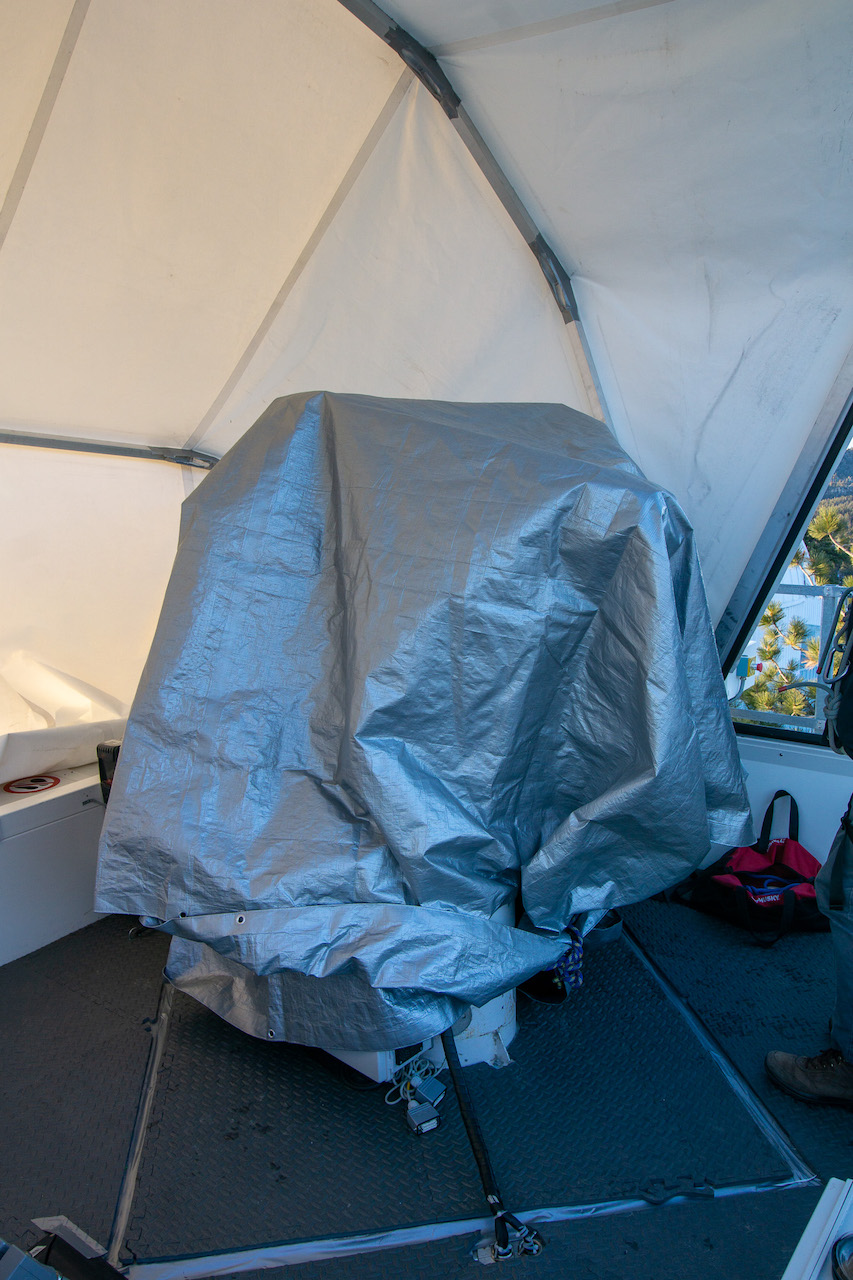
\includegraphics[width=0.65\linewidth]{figures/tarpaulin-coatlioan.jpg}
\end{center}
\caption{The telescope covered by a tarpaulin.}
\fi
\ifddotioan
\begin{center}
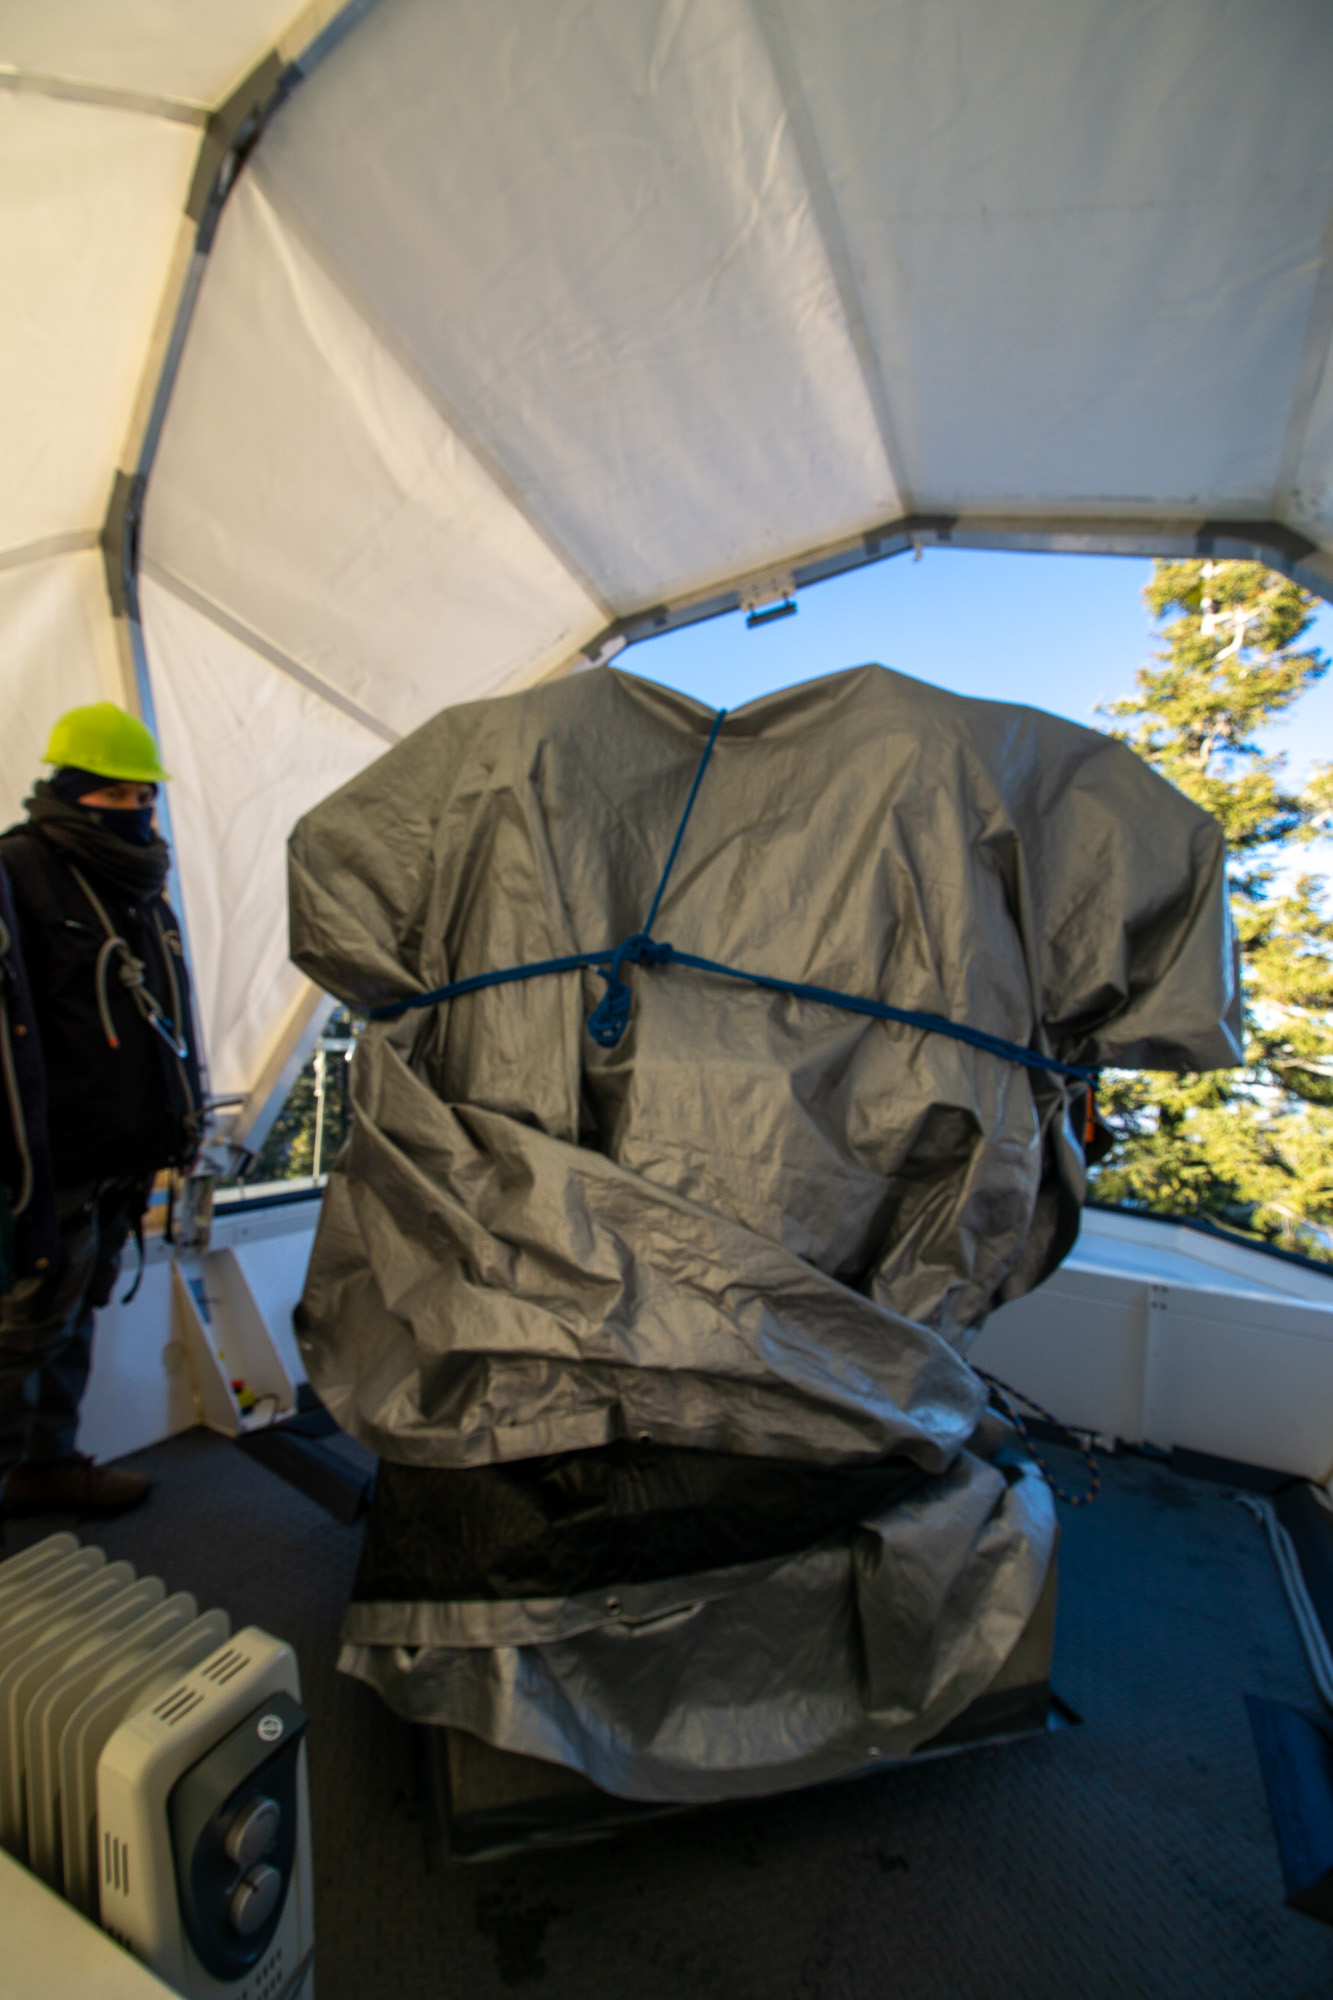
\includegraphics[width=0.45\linewidth]{figures/tarpaulin-ddotioan.jpg}
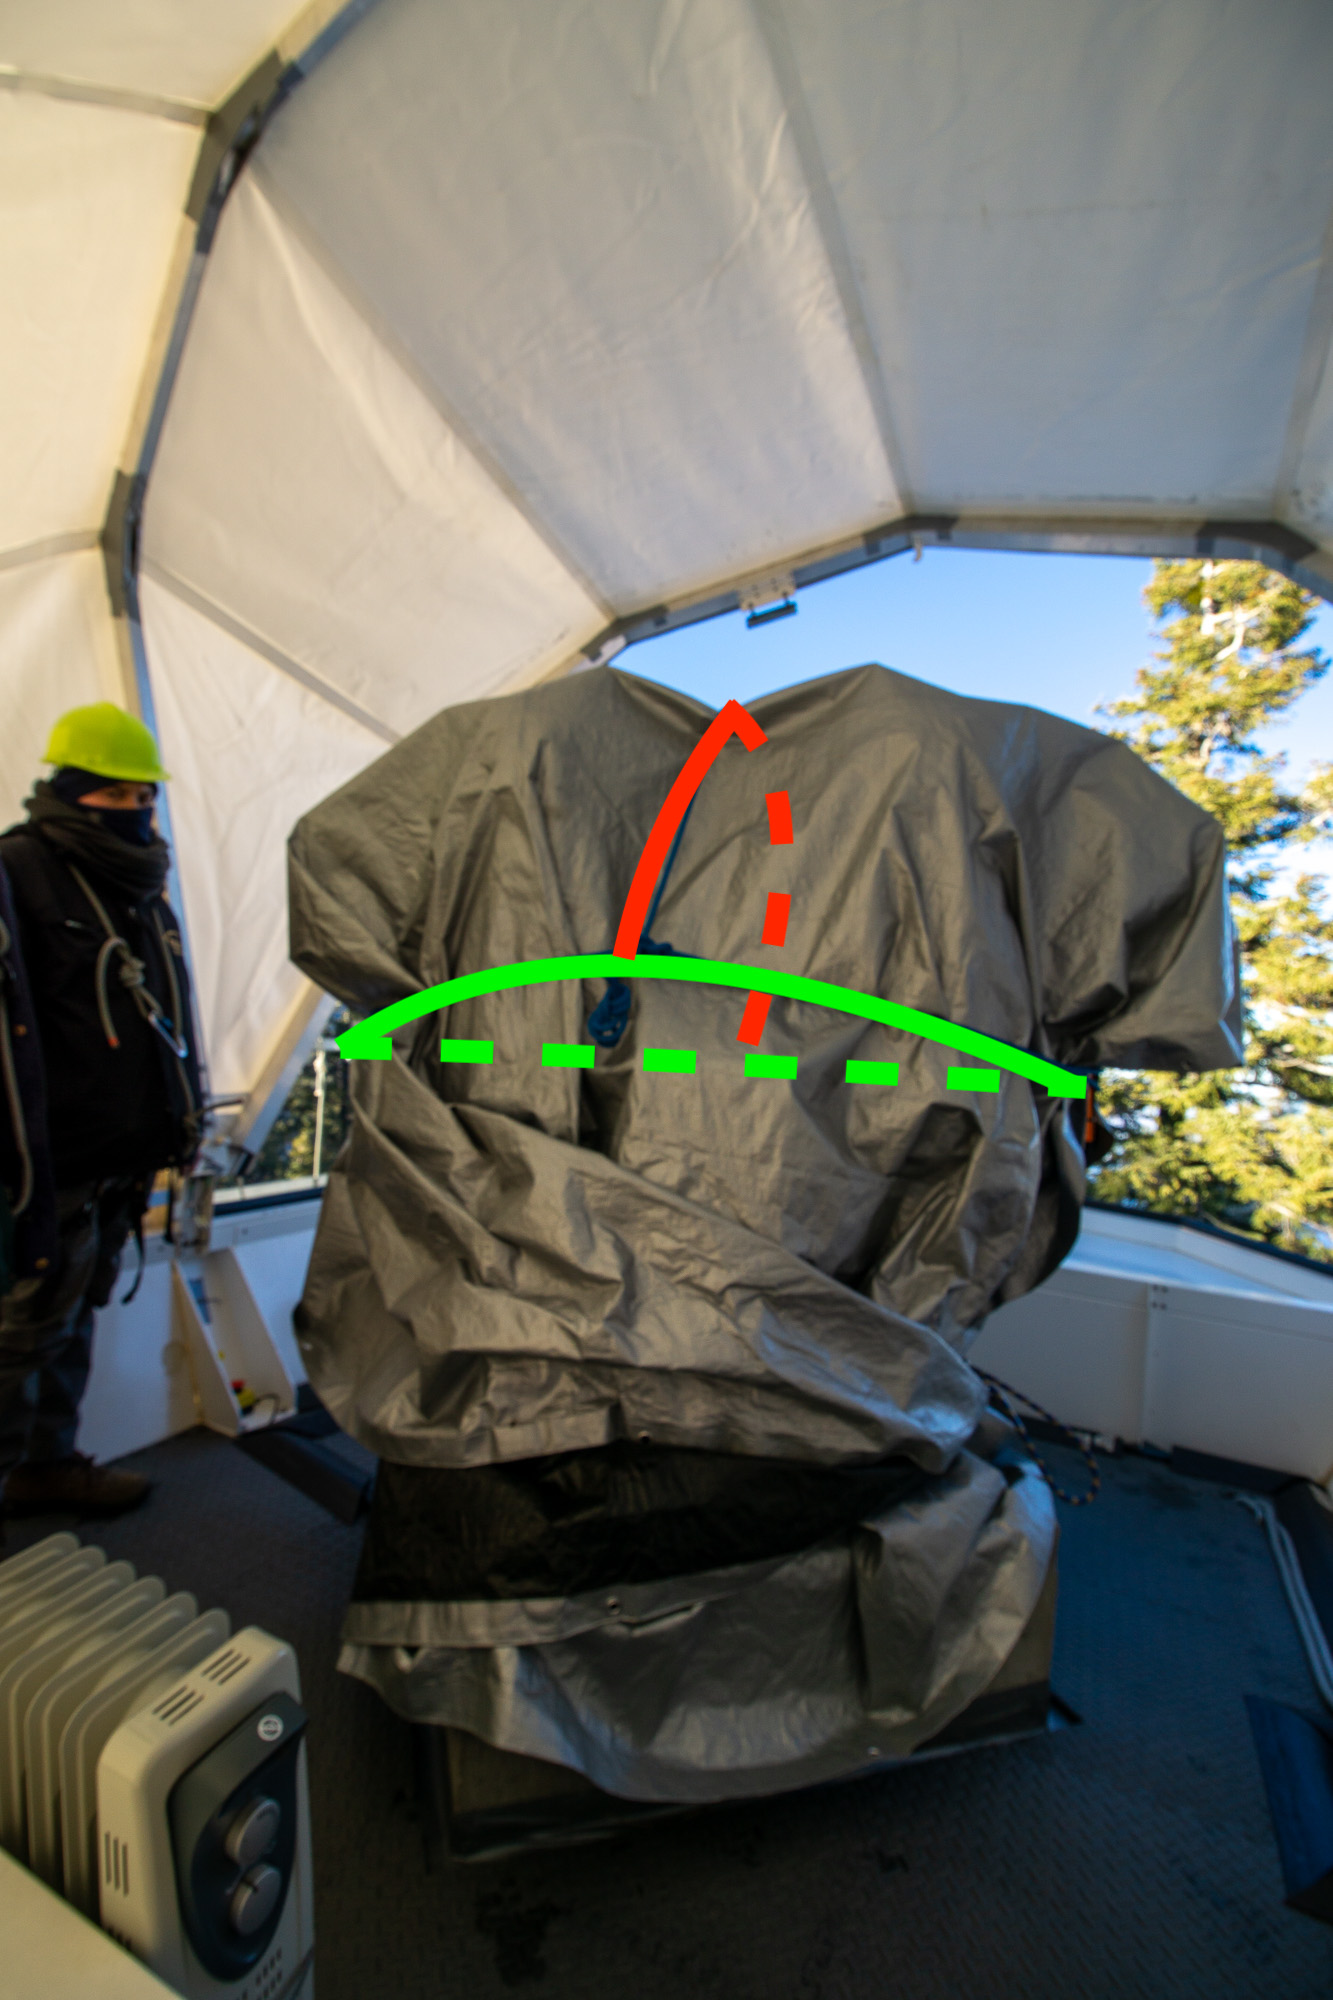
\includegraphics[width=0.45\linewidth]{figures/tarpaulin-ddotioan-annotated.jpg}
\end{center}
\caption{The telescope covered by a tarpaulin. The rope should go around the telescopes (green lines on the right, solid in front and dashed behind), below the two electronics boxes but above the lower end of the telescopes and the CCDs, and then over the the telescopes (red lines on the right), between the east and west sets, and fasten on itself to prevent it slipping down. The loose ends of the tarpaulin should be gathered and tied with a short red rope.  The tarpaulin and the ropes must not come into contact with the CCDs and must not place any stress on them.}
\fi
\label{figure:tarpaulin}
\end{figure*}

\item
Cover the telescope with a tarpaulin.
\ifcoatlioan
Gather the loose ends of the tarpaulin below and fasten them with a short red cord. See Figure~\ref{figure:tarpaulin}.
\fi
\ifddotioan
Be very careful not to place stress on the CCDs.

Wrap the long rope around the telescopes and tarpaulin, below the two electronics boxes but above the lower end of the telescopes and the CCDs, and then pass a loop over the telescopes, between the east and west sets, and fasten the rope on itself to prevent it slipping down. Gather the loose ends of the tarpaulin below and fasten them with a short red cord. See Figure~\ref{figure:tarpaulin}.

\emph{We repeat. The tarpaulin and the ropes must not come into contact with the CCDs and must not place any stress on them. The tarpaulin and ropes can only come into contact with the telescope tubes, focusers, and electronics boxes.}

\fi

\item
Descend from the platform.

\item 
Close the enclosure.

Press and hold the close button until the green light goes out.

\item
Switch off the enclosure controller.

Move the main power switch on the controller door from ON to OFF. (see Fig. \S\ref{figure:enclosure-controller-door}).
\item
Open the enclosure controller cabinet.

\item
Engage the manual lock. This switches on the enclosure electromagnet and actuates the enclosure emergency stop buttons. This ensures that the electromagnet stays energized even if the PLC fails and that the PLC cannot attempt to open the enclosure.

Move the manual lock switch inside the enclosure controller cabinet from OFF to ON. See Figure~\ref{figure:enclosure-controller-manual-lock-switch}.

\item
Close the enclosure controller cabinet.

\item
Switch on the enclosure controller.

Move the main power switch on the controller door from OFF to ON.

\item
Place the enclosure in remote mode.

Move the enclosure controller mode selector switch to “REMOTE”.

\item
\ifcoatlioan
Make sure the “PROHIBIDO EL PASO” sign is left in position at the bottom of the access stairs.
\fi
\ifddotioan
Make sure the “PROHIBIDO EL PASO” signs are left in position at the bottom of the access ladders.
\fi

\item
Leave the shed locked. Return the shed keys to the tool box (see \S\ref{section:shed}).

\end{enumerate}

\subsection{Soft Start-Up}
\label{section:soft-start-up}

\subsubsection{Safety Considerations}

\safety{You must use a safety harness, line, and helmet whenever you are on the  platform or balconies or to ascend the tower. Attach your line to one of the fasteners, to the balcony rail, or to something equivalently strong.} 

\safety{You must use a safety helmet if you are working under the platform or balconies.}

\safety{The enclosure controller cabinet uses 220 VAC. Switch off the power using the switch on the door before working inside the cabinet.}

\subsubsection{Requirements}

You will need:
\begin{itemize}
\item At least two persons.
\item The key to the shed (see \S\ref{section:shed}).
\item Weather conditions adequate for opening the enclosure and ascending to the platform.
\end{itemize}

\subsubsection{Procedure}

\begin{enumerate}

\item
In the shed, switch off the enclosure controller.

Move the main power switch on the controller door from ON to OFF.  (see Fig. \S\ref{figure:enclosure-controller-door}).

\item
Open the enclosure controller.

\item
Disengage the manual lock.

Move the manual lock switch inside the enclosure controller from ON to OFF. See Figure~\ref{figure:enclosure-controller-manual-lock-switch}.

\item
Close the enclosure controller.

\item
Switch on the enclosure controller.

Move the main power switch on the controller door from OFF to ON.

\item
Place the enclosure in local mode.

Move the enclosure controller mode selector switch to “LOCAL”.

\item
If the weather permits, open the enclosure to 60 deg.

Set the angle selector switch to 60 deg and then press and hold the open button until the green light goes out.

\item
Both persons should ascend to the platform.

\item
Remove the tarpaulin from the telescope.

\item Disengage the mount emergency stop button.

\item
\ifcoatlioan
Verify that the telescope is in the parked position, pointed at the northern horizon with the telescope on the west side of the pillar. If not, release the break on the mount by pressing the “BREAK” button and move it to this position.
\fi
\ifddotioan
Move the telescope to the parked position, pointed just below the northern horizon. To move the telescope, release the brake on the mount by pressing the “BRAKE” button.
\fi

\item Descent from the platform.

\item Close the enclosure. 

Press and hold the close button until the green light goes out.

\item
Place the enclosure in remote mode.

Move the enclosure controller mode selector switch to “REMOTE”.

\item
\ifcoatlioan
Make sure the “PROHIBIDO EL PASO” sign is left in position at the bottom of the access stairs.
\fi
\ifddotioan
Make sure the “PROHIBIDO EL PASO” signs are left in position at the bottom of the access ladders.
\fi

\item
Leave the shed locked. Return the shed keys to the tool box (see \S\ref{section:shed}).

\item
Store the tarpaulin in the shelves next to the cabinet in the 84-cm and the rope in the tool-drawer of the cabinet.

\end{enumerate}

\section{Hard Shut-Down and Start-Up}

A “hard” shut-down is appropriate for circumstances in which electrical power will not continue to be supplied to {\projectname}. This occurred, for example, in the evacuations for COVID-19. In this case, we must shut down the computers and cannot rely on the electromagnet to maintain the enclosure closed.

\subsection{Hard Shut-Down}

\subsubsection{Requirements}

You will need:

\begin{itemize}
    \item Two people plus the participation of a remote team member.
    \item The key to the shed (see \S\ref{section:shed-key}).
    \item Weather conditions adequate for opening the enclosure and ascending to the platform.
    \item The tarpaulin and ropes required for the soft shut-down (see \S\ref{section:soft-shut-down}).
    \item The two riveted plates, a riveter, and rivets.
\end{itemize}

\subsubsection{Procedure}

\begin{enumerate}
\item Perform a soft shut-down (see \S\ref{section:soft-shut-down}).
\item Communicate with the remote team member. They will:
\begin{enumerate}

   \item Log into a computer on the CU, Ensenada, or OAN networks of the Instituto de Astronomía (in order to gain ssh access to the firewall):
   
\begin{quote}\footnotesize
\begin{verbatim}
$ ssh user@somewhere.astrosxx.unam.mx -p 2222 -A -L 8080:localhost:8080
\end{verbatim}
\end{quote}

    \item Log into the firewall:
\begin{quote}\footnotesize
\begin{verbatim}
somewhere$ ssh user@ddoti.astrossp.unam.mx -p 2222 -A -L 8080:localhost:80
\end{verbatim}
\end{quote}

    \item Halt the computer \verb|access|:

\begin{quote}\footnotesize
\begin{verbatim}
firewall$ ssh user@10.0.1.2
access$ sudo shutdown -h -u now
\end{verbatim}
\end{quote}
    
    \item Switch off \verb|access| from \verb|ibb-127|.
\begin{quote}\footnotesize
\begin{verbatim}
firewall$ telnet 10.0.1.5
> get device #1
> set device #1 outlet <n> off
...
\end{verbatim}
\end{quote}
To log out of the iBootBar, use CTRL-] and then \verb|quit|.

    \item Halt the computers \verb|services|, \verb|control|, \verb|c0|, \verb|d0|, \verb|d1|, \verb|d2|, \verb|d3|, \verb|e0|, \verb|e1|, \verb|e2|, \verb|e3|:

\begin{quote}\footnotesize
\begin{verbatim}
firewall$ ssh ddoti@10.0.1.3
services$ sudo haltsoon
\end{verbatim}
\end{quote}

    \item Switch off \verb|instrument|, \verb|platform|, \verb|services|, \verb|control|, and \verb|mount| from \verb|ibb-127|.

\begin{quote}\footnotesize
\begin{verbatim}
$ ssh user@ddoti.astrossp.unam.mx -p 2222
firewall$ telnet 10.0.1.5
> get device #1
> set device #1 outlet <n> off
...
\end{verbatim}
\end{quote}
To log out of the iBootBar, use CTRL-] and then \verb|quit|.
    \item Halt the computer \verb|firewall|.

\begin{quote}\footnotesize
\begin{verbatim}
$ ssh user@ddoti.astrossp.unam.mx -p 2222 -L8080:localhost:80
\end{verbatim}

Open a browser to \verb|http://localhost:8080/| and halt the firewall from the web interface (select “Halt System” on the “Diagnostics” menu).
\end{quote}

\end{enumerate}

\item Switch off the two UPSes, the 127 V UPS and the 220 V UPS.

On both UPSes, press the power button on the front panel for three seconds. The UPS will start to beep and will then switch off.

\item Switch off the power supply to the two UPSes.

Open the breaker panel on the wall next to the door. Switch off circuits A and B.

\item
Install the two riveted two plates, one on each side of the enclosure, that hold it closed. See Figure~\ref{figure:riveted-plates}.

\begin{figure*}
\begin{center}
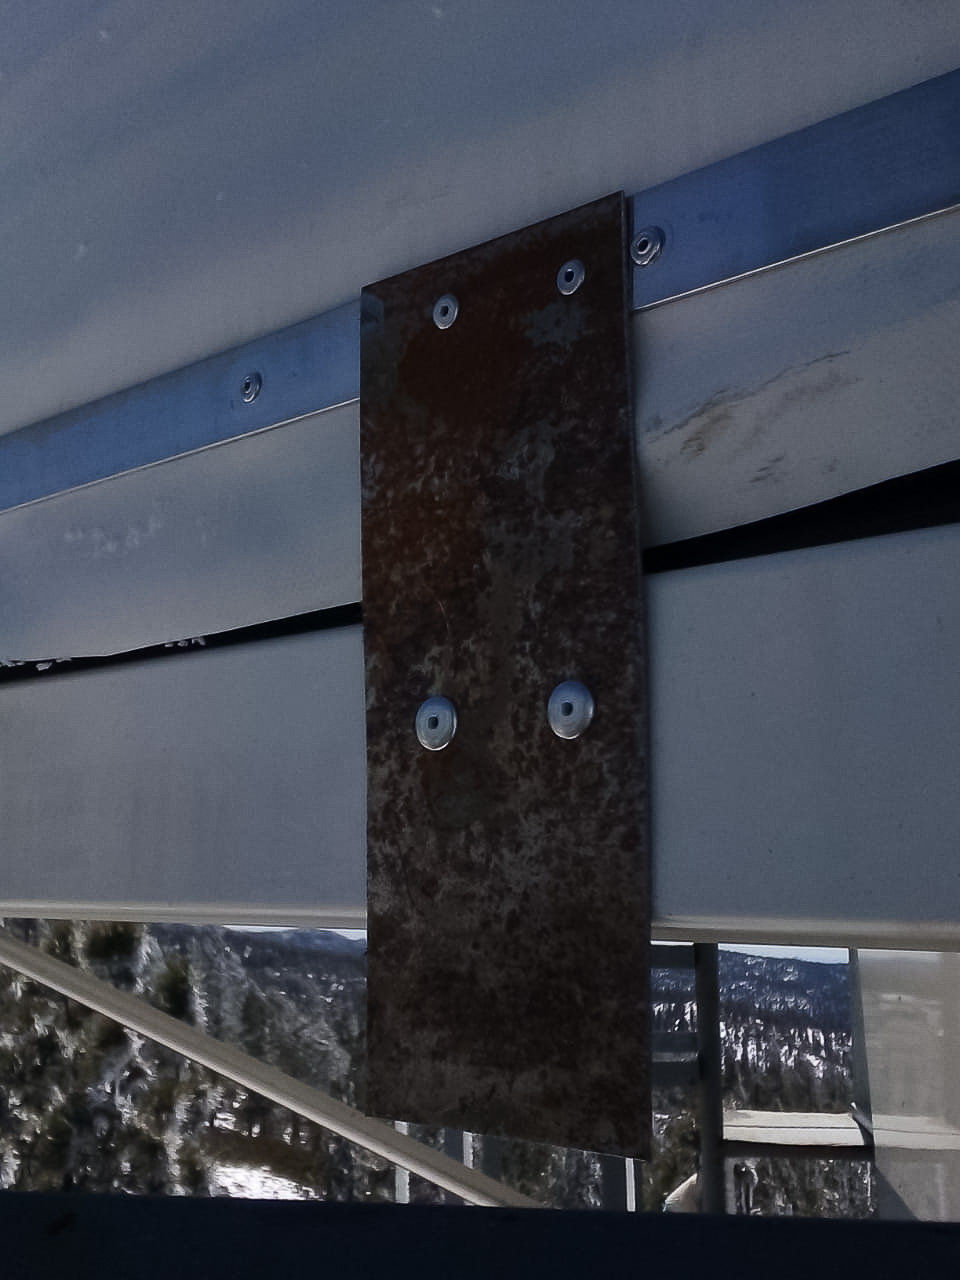
\includegraphics[width=0.45\linewidth]{figures/operations-riveted-plate.jpg}
\end{center}
\caption{One of the riveted plates that hold the enclosure closed when power is switched off.}
\label{figure:riveted-plates}
\end{figure*}

\end{enumerate}

\subsection{Hard Start-Up}

\subsubsection{Requirements}

You will need:
\begin{itemize}
\item At least two persons.
\item The key to the shed (see \S\ref{section:shed}).
\item Weather conditions adequate for opening the enclosure and ascending to the platform.
\item A drill (to remove the riveted plates).
\end{itemize}

\subsubsection{Procedure}

\begin{enumerate}
\item
Remove the two riveted two plates, one on each side of the enclosure, that hold it closed. See Figure~\ref{figure:riveted-plates}.

\item Switch on the power supply to the two UPSes.

Open the breaker panel on the wall next to the door. Switch on circuits A and B.

\item Switch on the two UPSes, the 127 V UPS and the 220 V UPS.

On both UPSes, press the power button on the front panel for at least one second.

\item Switch on the computer \verb|access|.

Press the button on the rear right of the computer.

\item Communicate with the remote team member. They will:

\begin{enumerate}
    \item Switch on the computers \verb|instrument|, \verb|platform|, \verb|services|, \verb|control|, and \verb|access| from \verb|ibb-127|.
    \item Verify that all of the computers boot.
\end{enumerate}

\item Perform a soft start-up (see \S\ref{section:soft-start-up}).

\end{enumerate}